% Chapter 3

\chapter{Évaluation et Feedback humain} 
\label{ch:3}

Bien que les \acp{llm} soient capables de restituer l'information avec une précision impressionnante, ils ne sont pas exempts d'erreurs et peuvent parfois produire des résultats erronés sous forme d'« hallucinations » \cite{zhu2024understanding, bai2024hallucination}. Ce terme désigne les instances où les modèles génèrent des contenus qui semblent plausibles mais qui ne sont pas fondés sur des faits réels ou vérifiables. Ces hallucinations peuvent inclure la fabrication de détails fictifs, la distorsion des informations existantes, ou l'émission de conclusions inexactes. Ce phénomène est particulièrement problématique dans le domaine juridique où la fiabilité et la précision des informations sont cruciales.

Étant donné notre objectif de vulgariser le Droit congolais de manière accessible et précise, il est impératif d'intégrer une couche d'évaluation humaine. Cette évaluation sera assurée par des professionnels du droit congolais, qui apporteront leur expertise pour vérifier et corriger les outputs du modèle. Leur rôle sera d'assurer que les informations générées par le chatbot soient non seulement correctes mais aussi pertinentes et utiles pour les utilisateurs finaux. Cette démarche permettra de pallier les limitations des \acp{llm} et de garantir que les informations diffusées respectent les normes juridiques et éthiques, renforçant ainsi la fiabilité et la crédibilité de notre projet.

L'intégration de feedback humain dans le processus d'évaluation contribue également à un cycle d'amélioration continue du modèle, où les corrections et les insights fournis par les experts peuvent être utilisés pour affiner et ajuster les algorithmes sous-jacents. Cette collaboration entre IA et expertise humaine est essentielle pour créer un outil robuste et fiable, capable de servir efficacement les besoins d'information juridique de la communauté.

\section{Critères et méthodes d'évaluations}

Dans une première phase d'évaluation, nous mettrons à l'épreuve les modèles existants en utilisant le test de magistrature congolais de 2022. Pour ce faire, nous appliquerons des critères d'évaluation rigoureux pour juger de la qualité des réponses générées par ces modèles. Ces critères sont les suivants :

\begin{enumerate}
    \item Pertinence : Nous évaluerons si les réponses fournies sont directement liées à la question posée et si elles traitent les aspects pertinents du cas juridique présenté. Il est crucial que chaque réponse aborde les éléments clés de la question pour être jugée pertinente.

    \item Clarté et Structure : La formulation des réponses doit être claire et compréhensible. La structure des réponses devra suivre une logique cohérente, facilitant ainsi la compréhension et la suivabilité des arguments.

    \item Analyse Juridique : Il est essentiel que les réponses démontrent une compréhension approfondie des principes juridiques impliqués. Nous attendons des analyses juridiques précises et adaptées au contexte du cas traité.

    \item Raisonnement et Logique : Les réponses doivent reposer sur un raisonnement solide et logique. Les arguments doivent être non seulement convaincants mais également bien développés pour soutenir les conclusions.

    \item Originalité et Créativité : Nous apprécierons les réponses qui offrent des perspectives originales ou des solutions créatives aux problèmes juridiques posés, ajoutant ainsi de la valeur à la simple restitution des faits ou des lois.
\end{enumerate}

Pour mener cette évaluation de manière objective, les réponses générées par les modèles seront collectées via un formulaire Google Form \footnote{\href{https://workspace.google.com/intl/en/products/forms}{https://workspace.google.com/intl/en/products/forms}}. De manière cruciale, les juristes chargés d'évaluer ces réponses ne sauront pas quel modèle a généré quelles réponses. Cette anonymisation est conçue pour prévenir tout biais dans l'évaluation, garantissant que les modèles sont jugés strictement sur la base de leur performance et non en fonction de leur notoriété présumée. 

\paragraph{Le test de magistrature 2022} \hspace{0pt}

\begin{longtable}{|p{0.7\textwidth}|p{0.3\textwidth}|}
\hline
\textbf{Question} & \textbf{Catégorie} \\
\hline
Peut-on constituer un prévenu gardien d'un objet saisi ? Dans la négative, donnez nous trois raisons. & procédure pénale \\
\hline
Les expressions, auteur présumé de l'infraction, l'inculpé, prévenu et condamné, traduisent quelles étapes des instances judiciaires. & procédure pénale \\
\hline
Quelle est la différence entre l'amnistie et la grâce du point de l'organe de décision ? & procédure pénale \\
\hline
Le ministère public peut-il requérir devant le juge le classement sans suite d'un dossier fixé devant le tribunal ? Dans la négative, donnez deux raisons. & procédure pénale \\
\hline
Le ministère public peut-il aussi introduire la procédure de suspicion légitime du tribunal dont il est membre de composition, si oui à quel titre. & procédure pénale \\
\hline
La nationalité congolaise peut-elle être détenue concurremment avec une autre nationalité par un sujet congolais vivant en \ac{rdc} ? Justifiez votre réponse. & droit civil des personnes \\
\hline
La dissolution du mariage par les autorités coutumières ou familiales peut-elle produire d'effets ? Justifiez votre réponse. & droit civil des personnes \\
\hline
Quelles sont les trois formes de testament consacré par la législation congolaise ? Explicitez-les. & droit civil des personnes \\
\hline
Monsieur FULANI marié à Madame SONGOLO décède en laissant derrière lui deux enfants nés avant le mariage, quatre enfants pendant le mariage, trois enfants hors mariage, un enfant adoptif, deux frères et trois soeurs. Le de cujus n'a laissé qu'un seul bien de valeur en l'occurrence un immeuble acheté auprès de l'ex ONL. L'aîné des enfants estime que le bien doit lui revenir. Les enfants nés pendant le mariage soutiennent qu'ils sont des enfants légitimes et peuvent seuls prétendre à l'héritage du de cujus. De leur côté, les frères et soeurs du défunt pensent que l'immeuble laissé par leur cadet ne doit revenir en priorité qu'à la famille. L'épouse du de cujus formule aussi les mêmes prétentions. S'agissant d'un seul bien de valeur, quelles solutions préconisez-vous à ces différentes prétentions ? & droit civil des personnes \\
\hline
Comment qualifie-t-on dans leur ordre progressif de degré de criminalité, les deux extrêmes de la tentative punissable ? & droit pénal général \\
\hline
Un condamné incarcéré à 12 heures du matin, pour subir un jour d'emprisonnement, constate dans sa fiche de libération qu'on l'a fait sortir le lendemain du jour d'incarcération à 14 heures, est-il en droit de se plaindre pour détention illégale ? & droit pénal général \\
\hline
En République Démocratique du Congo, la peine de fouet qui ne pouvait être infligée que par les juridictions indigènes a été supprimée par a- L'accession du Congo à l'indépendance le 30 juin 1960 b- L'accord global et inclusif du Sun City, après l'A.F.D.L. c- Le décret du 18 décembre 1951 avant l'indépendance & droit pénal général \\
\hline
Le calcul de jour de détention d'une personne incarcérée n commence-t-il : 
a- Le jour de la condamnation par le tribunal ? 
b-Le jour où la condamnation est coulée en force de chose jugée ? 
c- Le jour où sa détention est confirmée par la chambre de conseil ? 
d-Le jour où elle est placée sous mandat d'arrêt provisoire ? 
e-Le jour où elle a été privée de sa liberté ? & droit pénal général \\
\hline
En quoi l'amende judiciaire est différente de l'amende transactionnelle ? donnez au moins 4 points de différence. & droit pénal général \\
\hline

\caption{Questions du test de magistrature Congolais 2022}
\label{table:magisture-test-2022}
\end{longtable}

\newpage
\section{Évaluation des modèles existants}

Nous débuterons notre évaluation en attribuant à chaque modèle un identifiant anonyme afin de garantir l'impartialité de l'évaluation. Les modèles seront désignés comme suit : 

\begin{listing}[!ht]
\begin{minted}{python}
models = {
    'Modèle A': 'gpt3.5-turbo',
    'Modèle B': 'gemini-pro',
    'Modèle C': 'llama2',
    'Modèle D': 'mistral',
    'Modèle E': 'vicuna'
}
\end{minted}
\label{appendix:code:python:models}
\end{listing}

Après cette étape d'association, nous présenterons une série de questions issues du test de magistrature congolais de 2022 à chacun de ces modèles. Les réponses fournies par chaque modèle seront ensuite collectées et enregistrées au format \ac{csv} pour faciliter l'analyse et la comparaison ultérieures. voici un exemple pour le modèle gemini-pro \cite{geminiteam2023gemini} de Google :

\begin{listing}[!ht]
\begin{minted}{python}
import os
import google.generativeai as genai
import pandas as pd

genai.configure(api_key=os.getenv('GOOGLE_KEY'))
model = genai.GenerativeModel('gemini-pro')
questions = pd.read_csv('_magistrature.csv')

def generate_content(x):
    print(f"Answering question: {x['question']}")
    prompt = f"""
        Dans le contexte du Droit Congolais (RDC) précisément {x['category']},
        répondez à la question suivante : {x['question']}
    """

    response = model.generate_content(prompt)
    return response.text

questions['model'] = 'gemini-pro'
questions['answer'] = questions.apply(lambda x: generate_content(x), axis=1)
questions.to_csv('./data/answers-gemini-pro.csv', index=False)
\end{minted}
\caption{Évaluation du modèle Gemini Pro sur le test de magistrature 2022.}
\label{appendix:code:python:gemini-pro-evaluation}
\end{listing}

Chaque ensemble de réponses correspondant à un modèle sera également associé à une lettre, afin de préserver l'anonymat tout au long du processus d'évaluation. Cette méthode nous permet de suivre précisément quelle réponse appartient à quel modèle sans révéler cette information aux évaluateurs, assurant ainsi que les évaluations restent centrées uniquement sur la qualité des réponses par rapport aux critères établis, sans influence extérieure. 

\begin{figure}[H]
    \centering
    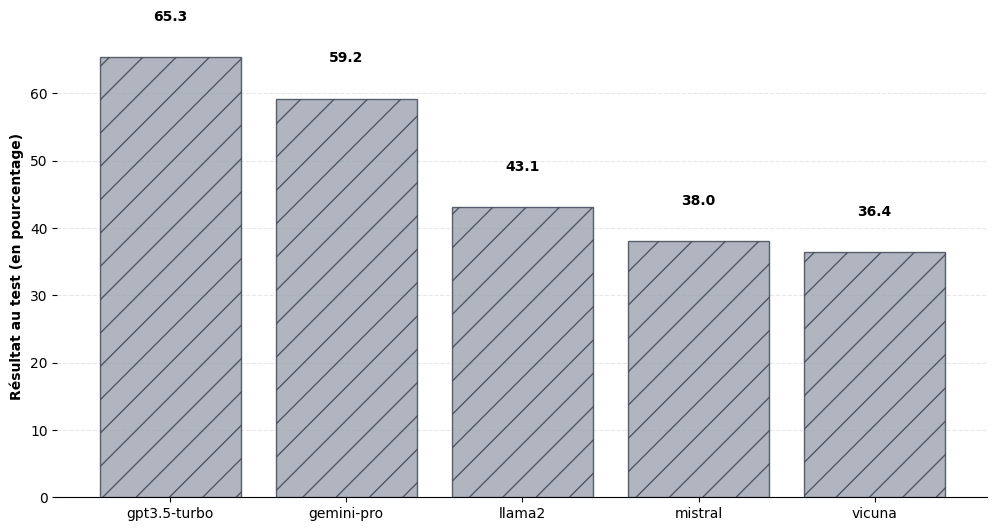
\includegraphics[width=15cm]{gfx/fig-model-result.png}
    \caption{Résultats après évaluation des différents modèles ,en pourcentage. (voir Code~\ref{appendix:code:python:model-result})}
    \label{fig:model-result}
\end{figure}


\newpage
\newpage
\section{Évaluation de notre modèle}


\section{Résultats et perspectives}
